\chapter{Review of relevant literature} \label{cha:Literature-review}

\section{Introduction} \label{sec:Lit-Review-Introduction}

There are two major fields of literature relevant to this project. Firstly, studies and technical reports delivered within engineering organisations relating to real spacecraft missions are examined, and compared to \BW. Secondly, there has been a long history of theoretical study into optimising spacecraft trajectories, from early impulsive spacecraft research to more recent low-thrust scenarios. A brief explanation of optimisation theory is provided, followed by a more in-depth investigation into recent application of these methods to low-thrust trajectory optimisation.

% -------------------------------------------------------- Past missions --------------------------------------------------------
\section{Past missions} \label{sec:Past-missions}

While \textcite{LePage1991} shows that there have been numerous Earth-orbiting satellites using electric thrusters for attitude control or station keeping, only a small number of spacecraft have ever escaped the Earth's sphere of influence using electric propulsion as the primary thrust. These are listed in \autoref{tab:Past-low-thrust-missions}, along with key specifications of their respective propulsion systems. Within the table, \emph{thrust} represents the maximum force that the primary propulsion system can exert on the craft. \emph{Power consumption} is the amount of electrical power used to operate at this maximum thrust. \emph{Specific impulse}, $I_{sp}$, is the momentum added by the thrusters per unit weight-on-Earth of propellant, and consequently represents the fuel efficiency of the thrusters. Electric propulsion is characterised by relatively high $I_{sp}$.

\begin{table}[ht]
\caption{Past low-thrust missions to escape Earth's sphere of influence}
\label{tab:Past-low-thrust-missions}
\centering
\begin{minipage}{\textwidth}
\begin{tabular}{C{0.2\textwidth} C{0.25\textwidth} C{0.2\textwidth} C{0.1\textwidth} c}\toprule
  Spacecraft & Propulsion type & Total Power \linebreak Consumption \linebreak (W) & Total Thrust \linebreak (mN) & $I_{sp}$ (s)\\\midrule
  DS-1\footnote{\textcite{web_DS-1}} & Electrostatic Ion Thruster & 2100 & 92 & 3300\\
  Hayabusa\footnote{\textcite{web_Hayabusa}} & $4\times$ Microwave ECR Thrusters & 1400 & 32 & 3200\\
  SMART-1\footnote{\textcite{web_SMART-1}} & Hall Effect Thruster & 1200 & 73 & 1640\\
  Dawn\footnote{\textcite{web_Dawn}} & Electrostatic Ion Thruster & 2100 & 90 & 3100\\\midrule
  Lunar Mission BW-1\footnote{\textcite{web_BW-1}} & $4\times$ Pulsed Plasma Thrusters & 220 & 4.9 & 2753\\
  & Thermal Arcjet & 801 & 103 & 486 \\\bottomrule
\end{tabular}
\end{minipage}
\end{table}

For the purposes of comparison, the Apollo program trans-lunar injection (TLI) was performed using a chemical propulsion system providing a thrust of approximately 1~MN (9 orders of magnitude greater than \BW) on a mass of 119,900~kg (only 3 orders of magnitude greater than \BW) at a specific impulse of 421~s. The Saturn V third stage that performed the TLI is shown at launch in \autoref{fig:SaturnV}.

\begin{figure}[ht]
\centering
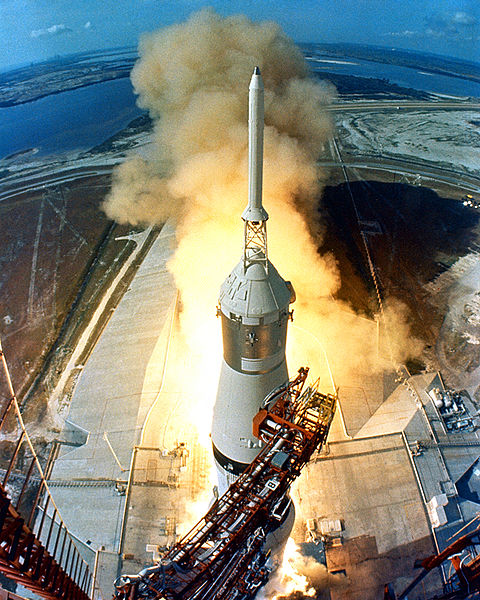
\includegraphics  [width=0.7\textwidth] {Images/Apollo_11_Launch2.jpg}
\caption{Saturn V from the Apollo program. Image used courtesy of \textcite{web_Apollo11}.}
\label{fig:SaturnV}
\end{figure}

\subsection{Deep Space One}
Deep Space One (DS-1), shown conceptually in \autoref{fig:DS-1}, was launched on 24 October 1998 with a mass of 374~kg \parencite{web_DS-1}. After launch, an electrostatic ion thruster took over propulsion on its one-way mission to the asteroid \emph{9969~Braille} and the comet \emph{19P/Borrelly}. This thruster generated 92~mN of thrust at a maximum input power of 2100~W. 

\begin{figure}[ht]
\centering
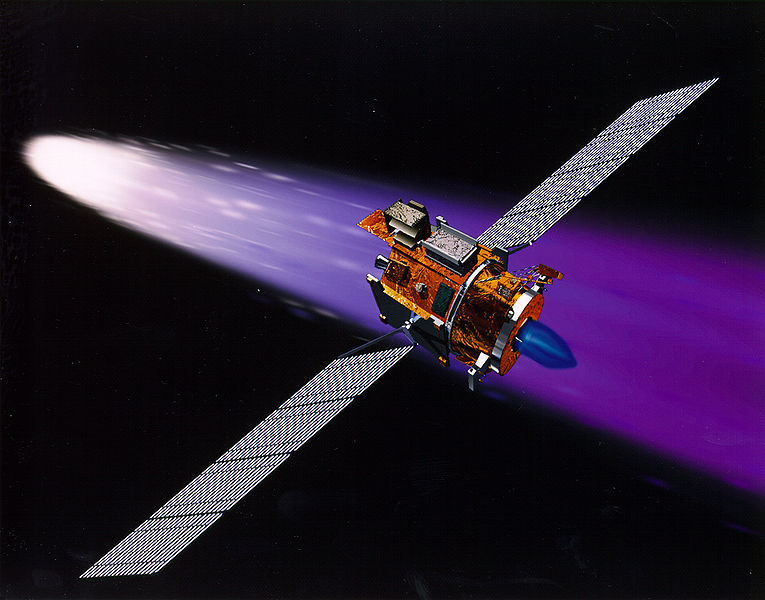
\includegraphics [width=0.7\textwidth] {Images/765px-Deep_Space_1_using_its_ion_engine.jpg}
\caption{Deep Space One. Image used courtesy of \textcite{web_DS-1}.}
\label{fig:DS-1}
\end{figure}
 
DS-1 had several similarities to the intended mission of \BW. \textcite{Rayman1997} state that once or twice each week the spacecraft had to rotate away from its thrust vector in order to collect optical navigation data and communicate with the Deep Space Network (DSN) on Earth, which required shutting down the propulsion system. Key differences from \BW\ however, include the frequency and duration of these thrusting and coasting phases, and the nature of the trajectory. The interplanetary trajectory of DS-1 was dominated by a heliocentric orbit, with perturbations from the Earth, Mars and a number of asteroids. This means that the thrust vector was almost tangential to the orbital velocity around the Sun, and therefore the optimal orientation of solar panels (towards the Sun) was always perpendicular to the desired thrust vector (around the Sun). In contrast to this, \BW\ will occupy a cis-lunar orbit. This poses two difficulties: not only will the trajectory optimisation have to switch its reference frame from Earth-centric to lunar-centric in mid-flight, but optimal orientation of the solar panels relative to the direction of thrust is constantly changing. To overcome this the thrusting profile of \BW\ must shut down much more frequently than DS-1 did: hourly, rather than weekly, so that it can point its solar panels towards the Sun to recharge.

\textcite{Rayman1999} provide a brief outline of the optimisation strategies used to design the DS-1 trajectory. A legacy in-house routine called the Solar Electric Propulsion Trajectory Optimization Program (SEPTOP) was used to determine an intial guess, implementing a calculus-of-variations optimisation technique. To reduce computational complexity, the heliocentric trajectory was constrained to month-long thrust arcs with a thrust vector fixed relative to a rotating frame. 
SEPTOP was then used to perform sensitivity analysis and to examine failure scenarios, before the coarse trajectory was then refined in a custom-built tool called the Computer Algorithm for Trajectory Optimization (CATO). This trajectory was then uploaded to the on-board navigation system AutoNav.

\subsection{Hayabusa}
Hayabusa (launched 9 May 2003), shown conceptually in \autoref{fig:Hayabusa}, was designed by the Japanese Aerospace Exploration Agency (JAXA) to perform a rendesvouz with asteroid \emph{25143~Itokawa} \parencite{web_Hayabusa}. It had a launch mass of 510~kg, including 130~kg of xenon gas used by the four microwave ECR (Electron Cyclotron Resonance) thrusters, providing 4$\times$8~mN = 32~mN thrust at maximum input power of 4$\times$350~W = 1400~W. 

Hayabusa had a similarly weak thrust to \BW, but was once again in a heliocentric orbit. Hayabusa successfully re-entered Earth's atmosphere and was recovered near Woomera, South Australia in June 2010, despite numerous failures including almost complete failure of all four ECR thrusters. The original trajectory design was published by \textcite{Masatoshi2003} in Japanese, but remains unverified due to the repeated major revisions required due to system failures.


\begin{figure}[ht]
\centering
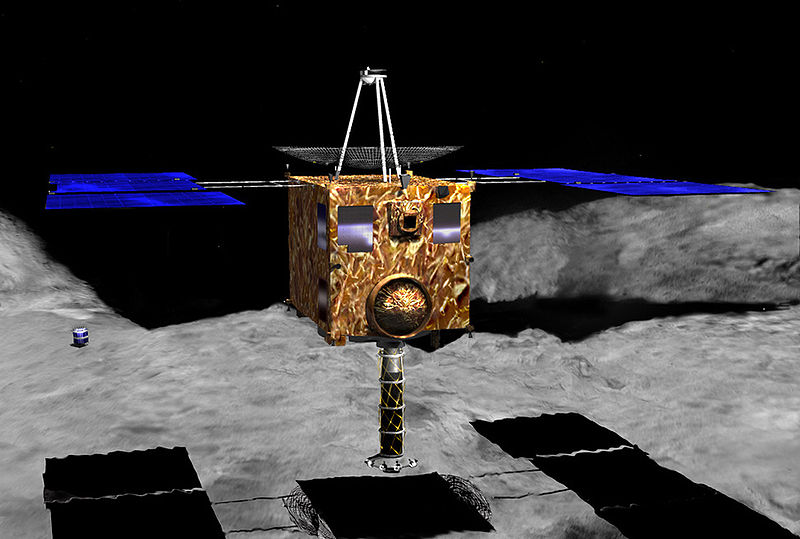
\includegraphics [width=0.7\textwidth] {Images/800px-Hayabusa_hover.jpg}
\caption{Japanese Hayabusa probe. Image used courtesy of \textcite{web_Hayabusa_NASA}.}
\label{fig:Hayabusa}
\end{figure}

\subsection{SMART-1}
Small Missions for Advanced Research in Technology One (SMART-1) (launched 27 September 2003) had a Hall effect plasma thruster providing 73~mN thrust at 1200~W power consumption \parencite{web_SMART-1}. The craft, shown conceptually in \autoref{fig:SMART-1}, was a comparable size to \BW, but twice as heavy: 367~kg including 80~kg of xenon propellant. On September 3, 2006 SMART-1 was deliberately crashed into the Moon's surface. This mission profile is closest to that intended for \BW, but had an order of magnitude higher thrust. 

\begin{figure}[ht]
\centering
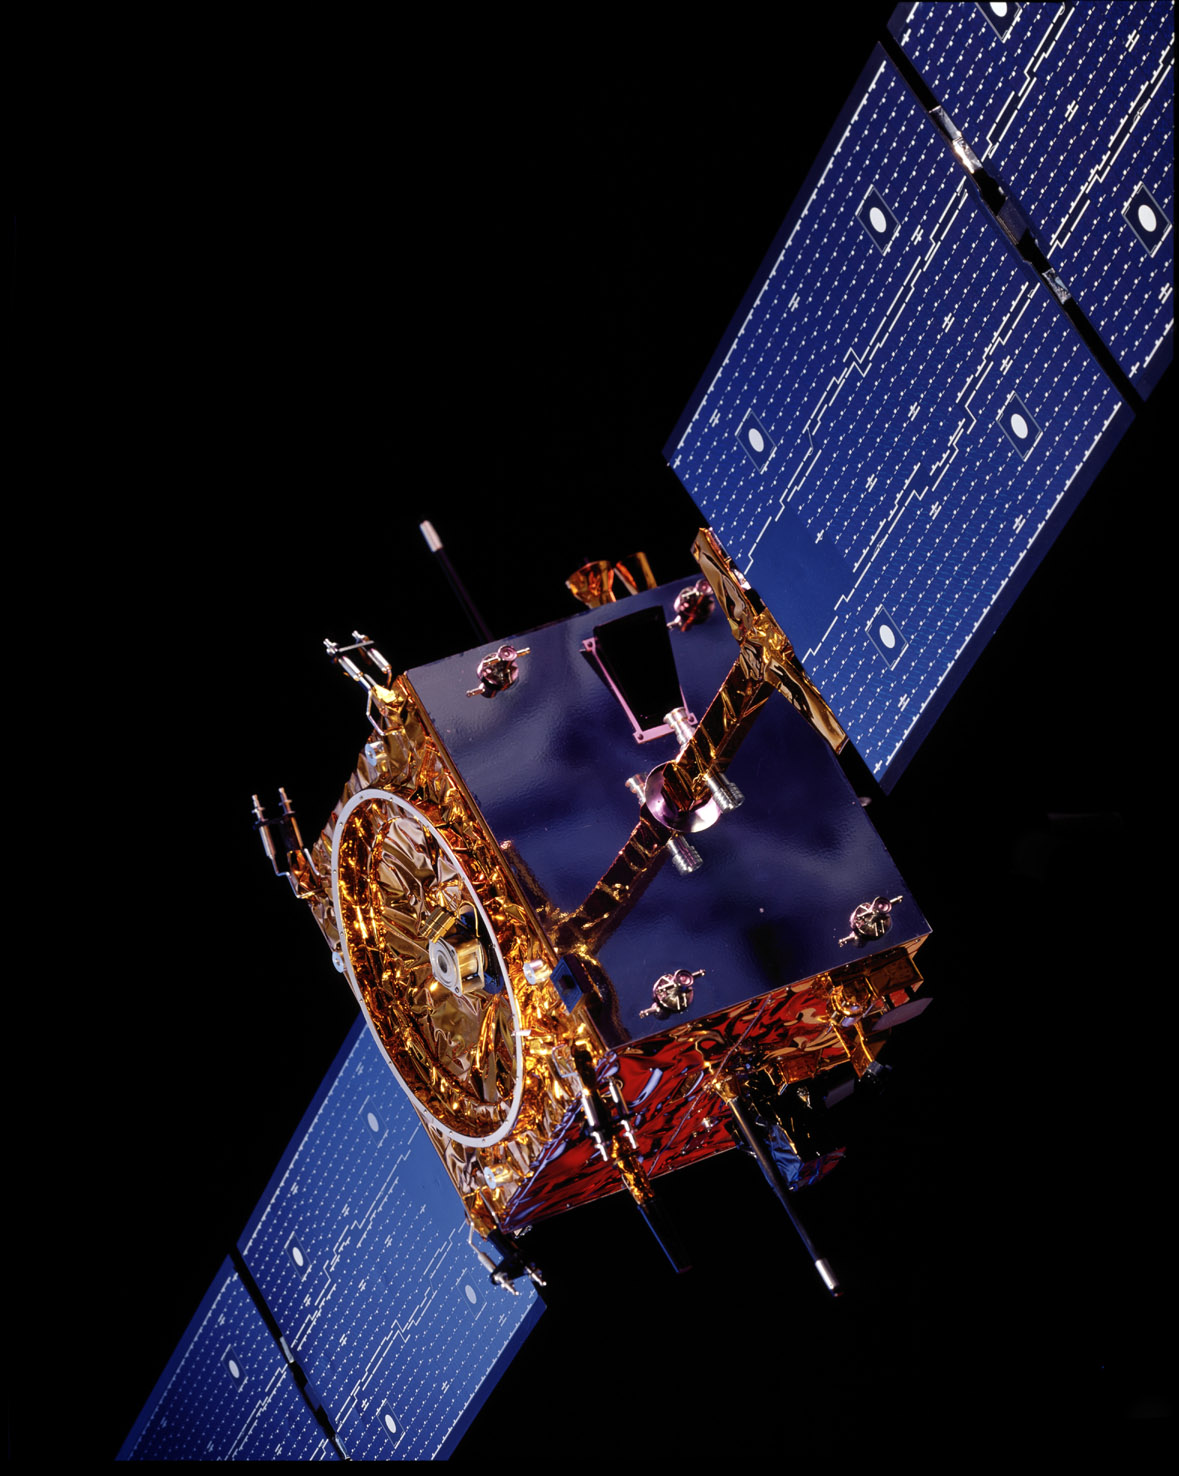
\includegraphics [angle=90,width=0.7\textwidth] {Images/SMART-1.jpg}
\caption{SMART-1. Image used courtesy of \textcite{web_SMART-1b}.}
\label{fig:SMART-1}
\end{figure}

Unlike \BW, SMART-1 had a mechanism to adjust the solar panel angle relative to the body to maximise incident sunlight. \textcite{Estublier2007} provides a useful summary of SMART-1 performance data, including that the GaAs solar panel performance started at 23.7\% efficiency, and decayed to 18-19\%. To allow continued thrusting during eclipse, Li-ion batteries were included allowing up to 2.1~hours of thrust. The Snecma PPS-1350G Hall effect thruster was mounted on a gimbal to allow reaction wheel unloading.

%also piggyback launch to GTO - could not set arg of periapsis, raan, incl etc.
%almost launch ideal conditions in late September - apogee near lunar ascending node

\textcite{Schoenmaekers2004} outlines the procedure and design factors influencing the trajectory design, but does not expound on optimisation methods used. Amongst a comprehensive summary of the entire mission and spacecraft design, \textcite{Racca2002} provides some information on the techniques used. SMART-1's first phase (GTO to 20,000~km periapsis) simply thrusted continuously along the orbital tangent. Phases 2 (cruise to 338,000~km apoapsis) was optimised using the Pontryagin maximum principle, by optimising the length of thrust and coast arcs within each orbit. Out-of-plane components were allowed, particularly during the higher orbits later in the phase, to perform a plane change. The third phase, incorporating the difficult lunar capture, utilised a gradient projection method to optimise a set of parameters defining the control law, thereby limiting the computational complexity of optimising a continuously variable thrust vector. Finally, the lunar descent from 60,000~km once again used the Pontryagin maximum principle to optimise the right ascension of the ascending node and arrival epoch of the final LLO, although thrust was constrained to the negative velocity vector thus severely limiting the computational complexity of the optimisation. Backwards integration was used to avoid the difficulties associated with lunar capture. 

\subsection{Dawn}
Dawn (launched 27 September 2007) is using the same thrusters developed for DS-1 to propel it towards the dwarf planet \emph{1~Ceres} by 2015 \parencite{web_Dawn}, following a successful rendezvous with the main-belt asteroid \emph{4~Vesta} in June 2011. Getting to Vesta it consumed 275~kg xenon, and will use another estimated 110~kg to get to Ceres, out of a total of 425~kg of on-board propellant. Dawn, shown conceptually in \autoref{fig:Dawn}, had a total launch mass of 1250~kg.

\begin{figure}[ht]
\centering
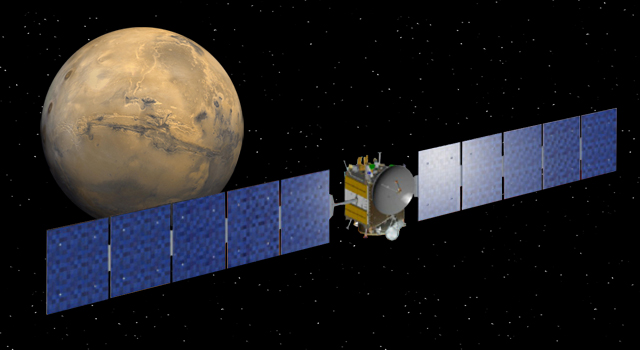
\includegraphics  [width=0.7\textwidth] {Images/mars-browse.jpg}
\caption{Dawn. Image used courtesy of \textcite{web_Dawn}.}
\label{fig:Dawn}
\end{figure}

Genetic algorithms and simulated annealing were investigated during Dawn mission planning \parencite{Lee2005a}, but the mission resorted to the same optimisation methods used by Deep Space-1 \parencite{Rayman2007}.

\subsection{Planned missions}
Planned electrically propelled missions include SMART-2, also known as LISA Pathfinder \parencite{web_SMART-2}, and Space-Technology~7 (ST-7) to be launched by NASA. Common to all of these missions is thrust substantially higher than \BW\ will have available, and consequently \BW\ will have a less flexible escape trajectory.

\BW\ will be only the fifth electrically propelled spacecraft to leave Earth orbit, and the first mission with this type of electric propulsion.
To increase its chances of success, a fuel-optimal trajectory must be sought.


% -------------------------------------------------------- Optimisation methods --------------------------------------------------------

\section{The process of optimisation} \label{sec:Optimisation-methods}

Optimisation is, intuitively, the process of finding an optimum value (minimum or maximum) for a given function. This is achieved by defining an \emph{objective function} or \emph{cost function} to rank results based on perceived value, allowing the result with the highest value to be chosen. The difficulty of performing optimisation arises from the potentially large number of results, and the difficulty of mathematically defining what is \enquote{good} or \enquote{bad}. 

% Generic definition
\subsection{Problem formulation} \label{sub:Formulation}

Typically, optimal control problems are formulated to find the required control history $\vec{u}(t)$ to deliver something (in this case, a vehicle) from an initial state $\vec{x}(t_0)$ to a final state $\vec{x}(t_f)$ while minimising the cost function $F$, where $t$ is some smoothly increasing or decreasing parameter. 

Along with the control history there are several other parameters (such as departure date, slackness within the initial and final conditions, and phase lengths) that make up the optimisable parameter set $\vec{p}$. The generic optimisation problem is
\begin{equation} \label{eq:Optimisation}
\min F(\vec{u}(t),\vec{p}).
\end{equation}
This optimisation is, of course, subject to certain equality constraints $g_{eq}$ and inequality constraints $g_{ineq}$ which depend on the state $\vec{x}$, control parameters $\vec{u}$, optimisable parameters $\vec{p}$ and independent parameter $t$, 
\begin{subequations} \label{eq:Constraints}
\begin{align}
g_{eq}(\vec{x}(t),\vec{u}(t),\vec{p},t) &= 0, \\
g_{ineq}(\vec{x}(t),\vec{u}(t),\vec{p},t) &\ge 0.
\end{align}
\end{subequations}
The differential equation \eqref{eq:generic-DE} then describes how the state evolves over the trajectory,
\begin{equation}\label{eq:generic-DE}
\frac{d\vec{x}}{dt} = f(\vec{x}(t),\vec{u}(t),\vec{p},t).
\end{equation}

For computational reasons (see \autoref{sub:Scaling}), upper and lower bounds are supplied for the states, controls and optimisation parameters,
\begin{subequations} \label{eq:Bounds}
\begin{gather}
\vec{x}_l\le\vec{x}(t)\le\vec{x}_u \label{eq:state-bounds}, \\
\vec{u}_l\le\vec{u}(t)\le\vec{u}_u \label{eq:control-bounds}, \\
\vec{p}_l\le\vec{p}\le\vec{p}_u \label{eq:parameter-bounds}.
\end{gather}
\end{subequations}

The cost function $F$ must be defined with the same parameters, but may include components evaluated at the start of the trajectory, end of the trajectory, and integrated over the trajectory, added together with appropriate weighting factors $\sigma$,
\begin{subequations} \label{eq:cost-function}
\begin{gather}
F_0=f(\vec{x}(t_0),\vec{u}(t_0),\vec{p},t_0) \label{eq:init-cost}, \\
F_f=f(\vec{x}(t_f),\vec{u}(t_f),\vec{p},t_f) \label{eq:final-cost}, \\
F_i=\int^{t_f}_{t_0}f(\vec{x}(t),\vec{u}(t),\vec{p},t)\quad dt \label{eq:integral-cost}, \\
F = \vec\sigma_0 F_0+\vec\sigma_f F_f+\vec\sigma_i F_i \label{eq:total-cost},
\end{gather}
\end{subequations}
where the subscripts $0$, $f$, and $i$ represent initial, final and integrated cost functions, respectively.


% Trajectory propagation
\subsection{Trajectory propagation} \label{sub:Propagation}
The path between initial and final states is defined by a differential equation of motion as outlined in equation \eqref{eq:generic-DE}. A number of numerical methods are available for approximating the solution to differential equations such as these. In general, the gradient at some starting point is used to estimate another point a small distance away. Most common are the Runge-Kutta methods, which use an iterative estimate of the gradient at the midpoint to get a more accurate estimate for the endpoint. The fourth order Runge-Kutta method for $y'=f(t,y)$ is calculated by
\begin{subequations} \label{eq:RK4}
\begin{gather}
y_{n+1}=y_n+\frac{1}{6}\left(k_1+2k_2+2k_3+k_4\right), \\
k_1=hf\left(t_n,y_n\right), \\
k_2=hf\left(t_n+\frac{h}{2},y_n+\frac{k_1}{2}\right), \\
k_3=hf\left(t_n+\frac{h}{2},y_n+\frac{k_2}{2}\right), \\
k_4=hf\left(t_n+h,y_n+k_3\right),
\end{gather}
\end{subequations}
where $h$ is the step size \parencite{recipes}. A similar, commonly used method in optimal control is Hermite-Simpson interpolation \parencite{recipes}.

Adaptive Runge-Kutta methods use the difference between two fixed-step Runge-Kutta methods to place bounds on the accuracy of the estimated endpoint. If the accuracy is not within some predefined tolerance, the interval size is revised. Particular care must be taken when integrating a non-linear differential equation over an extended duration such as the \BW, due to the accumulation of numerical errors.

%\subsection{Integration techniques} \label{sub:Integration}

Regardless of the numerical method used, trajectory optimisation requires solving the differential equations over a span of time; low-thrust trajectory optimisation requires very long timespans. Every integration step is associated with a potential error, which accumulates over the timespan. Methods that integrate from the start to the finish, termed \emph{direct shooting} or \emph{single shooting} methods, become increasingly error-prone as the timespan increases. Small changes early in the trajectory create large changes later on, which can make the constraints behave very non-linearly \parencite{Betts1998}. 

If some intermediate states can be reliably guessed, the integration may be started anew from that \enquote{node}. Any discontinuity at the node is added to the set of constraints, resulting in a relatively larger number of optimisation variables. Methods that perform multiple independent integrations like this, termed \emph{multiple shooting} methods, are less prone to integration error, but convergence is heavily dependent on the accuracy of the intermediate state guesses \parencite{Betts1998, ASTOS_guide}. Consequently, many multiple shooting methods now incorporate automatic initial guess estimation. Multiple shooting is sometimes called \emph{parallel shooting}, because each segment may be calculated in parallel. This method therefore lends itself well to parallel processing, across multiple core processors or even clusters of networked computers. 

Finally, to reduce computational complexity the changes in control and/or state over time may be approximated by a piecewise linear or polynomial function. Any algorithm that uses a simplification like this is said to solve the \emph{parameterised optimal control problem}. If the algorithm approximates control and state nodes at the same points, it is a \emph{collocation} method. Since this reduces the number of nodes required, collocation is generally faster than multiple shooting, but not as accurate.%cite


% Optimisation 
\subsection{Optimisation methods} \label{sec:Process}

Any trajectory propagated as in \autoref{sub:Propagation} that satisfies the boundary value problem stated in \autoref{sub:Formulation}, within acceptable error bounds, is a potential solution to the optimal control problem. These solutions may then be ranked using the objective function presented in equation \eqref{eq:cost-function}. The remaining task is to evaluate enough potential solutions to be confident that the highest scoring one is indeed optimal. 

There are two general approaches to this problem, classified consistently across literature such as \textcite{Betts1998} and \textcite{ASTOS_guide}. \emph{Indirect methods} attempt to solve the derivative of the cost function and thus determine a stationary point in the function space. \emph{Direct methods} simply evaluate the cost function at a number of nearby points in the function space, and repeat the process from the best solution found. Once no adjacent points in the function space possess better costs, an optimum has been attained. Both of these methods satisfy the necessary and sufficient conditions of an optimum. 

\subsubsection{Necessary and sufficient conditions} \label{sub:Neccessary-and-sufficient}

Pierre de Fermat first proved that optima of unconstrained problems are found at stationary points in the objective function \parencite{Fermat}. The addition of inequality constraints adds some complexity in that the global optimum may be located on the edge of the acceptable set; that is, where an active constraint disallows any points deeper along the gradient. These constraints may be appended to the objective function to form a \emph{Lagrangian}, which modifies the overall problem into an unconstrained set. Because this test requires the gradient or first derivative of the Lagrangian (called the \emph{Jacobian}) to be calculated, it is called a \emph{first order condition}. Satisfying the first order condition is necessary for the point to be a local optimum.

While the first order test identifies points that might be optima, it does not disinguish a minimum from a maximum or an inflection point. When the objective function is twice differentiable, these cases can be distinguished by checking the second derivative (the gradient of the gradient, called the \emph{Hessian}). The conditions that distinguish maxima, or minima, from other stationary points are called \emph{second order conditions}. If a candidate solution satisfies the first order conditions, then satisfaction of the second order conditions is sufficient to establish at least local optimality.

Indirect methods rely on these tests to determine search direction. Direct methods include these tests implicitly by adjusting the search space towards the most favourable solution (consequently along the steepest gradient) until there is no more favourable solution nearby (the gradient is zero). If the second order test were not satisfied, better solutions would be found adjacent to the candidate solution. Both types of methods require evaluation of the Lagrangian.

% Lagrangian
\subsubsection{Lagrangian} \label{sub:Lagrangian}

As mentioned above, %in \autoref{sub:Neccessary-and-sufficient}, 
adding the constraints to the cost function transforms the constrained problem into an unconstrained problem. The resulting cost function is known as the Lagrangian, $\mathcal{L}$, and is defined as
\begin{equation} \label{eq:Lagrangian}
\mathcal{L} = F(\vec{u}(t),\vec{p}) - \sum\lambda g_{eq}(\vec{x},\vec{u},\vec{p},t) - \sum\mu g_{ineq}(\vec{x},\vec{u},\vec{p},t),
\end{equation}
where the cost function $F$ was explained in \autoref{sub:Formulation}. The Karush-Kuhn-Tucker (KKT) multipliers, $\lambda$ and $\mu$, are added to the set of optimisable parameters, and subject to additional constraints ($\lambda_i\ge0$ and $\mu_i\ge0$ for all $i$). This forms the \emph{complementary slackness condition}. For any feasible solution, the equality constraints and active inequality constraints will give $g(\vec{x})=0$.  Since the inactive inequality constraints $g(\vec{x})>0$, their respective KKT multipliers will be driven down to improve the Lagrangian until $\lambda=0$. Therefore, minimising the Lagrangian minimises the objective function and ensures all constraints are met.

% Indirect methods
\subsubsection{Indirect methods}

%As introduced in \autoref{sub:Neccessary-and-sufficient}, indirect methods 
Indirect methods attempt to solve the optimal control problem by finding a stationary point in the solution space that satisfies the second order condition of being an optimum. Traditionally this is achieved analytically through the calculus of variations, using Pontryagin's minimum principle \parencite{Pontryagin1962}. 

%This states that optimising the Hamiltonian of a system is a necessary condition for the optimal control of that system. As shown by \textcite{Ren2007}, generating the Hamiltonian for the modified equinoctial elements is simple, by placing equation \eqref{eq:state-updates} in the form $\dot{\vec{x}}=\mathbf{B}\Delta+\vec{d}$
%here the state variable $\vec{x}=\left[\begin{array}{cccccc} p & f & g & h & k & L\end{array}\right]^{T}$
%consists of the equinoctial element set defined in Section \ref{sec:Orbital-Elements}, $\mathbf{B}$ is a $3\times6$ matrix that represents the thrust coefficients, and $\vec{d}=\left[\begin{array}{cccccc} 0 & 0 & 0 & 0 & 0 & D\end{array}\right]^{T}$
%where $D=\sqrt{\mu p}\left(\frac{w}{p}\right)^{2}$ and represents the natural circular motion (zero thrust trajectory).
%The Hamiltonian is then %need to define terms here too, 
%$\lambda,\lambda_{L},\lambda_{m},m$
%\begin{equation}
%H=\vec{\lambda}^{T}\mathbf{B\Delta}+\lambda_{L}d-\lambda_{m}\frac{T}{I_{sp}g_{0}}\label{eq:hamiltonian}
%\end{equation}
%with costate equations
%\begin{equation}
%\dot{\vec\lambda}=-\frac{\delta H}{\delta\vec{x}}=-\vec{\lambda}^{T}\frac{\delta\mathbf{B}}{\delta\vec{x}}\Delta-\lambda_{L}\frac{\delta d}{\delta\vec{x}}\label{eq:lambda_dot}
%\end{equation}
%\begin{equation}
%\dot{\lambda}_{m}=-\frac{\delta H}{\delta m}=\vec{\lambda}^{T}\mathbf{B}\frac{\mathbf{\Delta}}{m}=\left\Vert \vec{\lambda}^{T}\mathbf{B}\right\Vert \frac{T}{m^{2}}\label{eq:lambda_m_dot}
%\end{equation}

% explain what is done once the Hamiltonian is optimised

Pontryagin's minimum principle requires solution of the adjoint equations. % define adjoint equations?
The existence of an analytical solution consequently becomes highly dependent on the linearity of the adjoint equations, but assumptions and simplifications can sometimes be made in order to determine a general solution to the equations. These assumptions are usually only valid for short duration scenarios such as the missile trajectory described by \textcite{Ohlmeyer2006} and the re-entry of the two exo-atmospheric stages of the Saturn~V rocket presented by \textcite{Haeussermann1965}. Given the long durations and non-linearities present in low-thrust trajectories, an analytical solution usually cannot be found.

An alternative to solving the infinite-dimensional optimal control problem is to discretise the problem and solve the resulting high- but finite-dimensional problem using indirect numerical methods. Forgoing a general solution to the objective function, these methods break the problem down into many sub-problems, each of which may be solved locally. This is collectively known as nonlinear programming (NLP) \parencite{Betts1998}. 

The general approach to nonlinear programming is take a candidate solution, $\vec{x}_0$. An iterative procedure is then used to improve this solution by varying the state a certain amount, $\alpha$, in a certain direction, $\vec{k}$, as defined in equation \eqref{eq:NLP}. The sign of the step direction, $\alpha$, determines whether the algorithm finds a minimum or a maximum,
\begin{equation} \label{eq:NLP}
\vec{x}_{n+1}=\vec{x}_n+\alpha\vec{k}.
\end{equation}

\textcite{Gauss1827} pioneered gradient-based methods in the early 19th century, by using the Jacobian of the Lagrangian with respect to the state vector, $\nabla\mathcal{L}$, as the search direction,
\begin{equation} \label{eq:gradient-method}
\vec{x}_{n+1}=\vec{x}_n + \alpha\nabla\mathcal{L}(\vec{x}_n).
\end{equation}
This technique is also known as the method of steepest descent, because the Jacobian matrix functions as a multi-dimensional gradient. When a candidate solution is found with no gradient that leads to a better solution, the candidate solution must be a local optimum.

Pure gradient methods are prone to slow optimisation, particularly with stiff problems. %define stiff problems, cite
A second-order variant on this scheme is often referred to as \emph{Newton's method} because it uses the iterative root-finding scheme devised by \textcite{Newton1711, Newton1736} to determine the zeroes of the gradient. Since the gradient is itself a derivative of the Lagrangian, this technique requires computation of a second derivative, 
\begin{equation} \label{eq:newtons-method}
\vec{x}_{n+1}=\vec{x}_n + \alpha\frac{\nabla\mathcal{L}(\vec{x}_n)}{\nabla^2\mathcal{L}(\vec{x}_n)}.
\end{equation}
The curvature information held within the second derivative matrix (called the Hessian matrix, $\nabla^2\mathcal{L}$) allows this technique to converge faster, but each iteration takes more computational effort.

Various schemes exist to calculate the step size, $\alpha$. These algorithms, collectively called a \emph{line search}, can often be very computationally inefficient and time consuming. When the step size, $\alpha$ is equal to one, gradient methods assume a linear behaviour in the vicinity of the candidate solution, and select the next iteration accordingly. Newton's method assumes a quadratic behaviour in the vicinity. Variations on Newton's method have been used to great success in many optimisation applications, not least trajectory optimisation, leading to the techniques being collectively named \emph{sequential quadratic programming} (SQP). Quasi-Newton methods such as the Broyden-Fletcher-Goldfarb-Shanno (BFGS) method use an approximation of the Hessian to speed up computation while retaining the benefits of second-order gradient information. 

In certain applications such as low thrust trajectories, the long propagation times requiring many grid points result in very large, sparse Jacobian and Hessian matrices. A sparse matrix is characterised by very few non-zero terms \parencite{Stoer2002}, due to very loose coupling; changes early in the trajectory do not have a direct effect on the later stages of the trajectory except by influencing all of the intervening states. Some algorithms are able to exploit this sparsity to calculate the Hessian and Jacobian matrices very efficiently.

% John von Neumann developed an alternative to gradient methods, known as the \emph{interior point method}...

%can perhaps use \cite{Well2001} for reference about GESOP, SQP, collocation, direct shooting
%\textcite{Nocedal2006} basic intro to optimisation

%A useful measure of stiffness is the condition number of the Hessian matrix. A high condition number means the system is very sensitive to small changes in the perturbation vector. During optimisations conducted for this project, the condition number was often of the order $10^{11}$, demonstrating the stiffness of this problem.


% Direct methods
\subsubsection{Direct methods}

Direct methods, in contrast to indirect methods, do not try to determine additional information from the objective function. They simply evaluate the objective function at a number of points, and then adjust the search space towards the best solution found. Consequently direct methods cannot be analytical. %However, the resulting direct numerical methods rely on the same principles as indirect numerical methods, so the general optimisation scheme presented in equation \eqref{eq:NLP} is still valid. 

There are many different techniques to determine which solutions to evaluate. A number of techniques, such as tabu search and hill-climbing, merely search adjacent solutions and consequently function only as local search methods. Without using gradient information each iteration must exhaustively search the adjacent function space, so these techniques are less efficient than indirect methods (subject to the difficulty of gradient computation). The real advantage of direct methods emerges when each iteration is allowed to search a wider space.

The largest group of direct methods is evolutionary algorithms. In general, these techniques evaluate a number of candidate states, make a few random changes and then re-evaluate the new generation, picking the best solutions to continue with. For example, genetic algorithms avoid local minima by performing random mutations and genetic crossovers, emulating the biological process of evolution. Another example called simulated annealing was introduced by \textcite{Kirkpatrick1983}, and emulates a blacksmithing technique where the metal is cooled slowly to allow the particles to align into an optimised (crystallised) low energy state. 

Evolutionary algorithms are heavily dependent on their implementation, and the efficiency of their mutations, to steer the evolution of the solution. Furthermore, with delicate problems such as \BW, random mutations frequently lead to invalid solutions (the spacecraft does not reach the target orbit) and consequently these techniques can struggle to find alternative feasible solutions, as changes may be required to multiple parameters before another basin of convergence is found.

Another group of direct methods is called dynamic programming. These techniques are particularly used in financial programming and management science, with the aim of finding the path of least cost in a discrete system by evaluating each step backwards from the goal using the recursive Bellman equations \parencite{recipes}. As such dynamic programming is best suited to heavily discretised states and paths between states, and consequently a very limited number of controls. Dynamic programming has been expanded to solve continuous time problems using the Hamilton-Jacobi-Bellman equations, but this adaptation requires calculation of the cost function gradient, converting the technique to an indirect method \parencite{recipes}.

% Memetic algorithm - like genetic algorithms with memes
% Differential evolution - another algorithm to create next generation [a + F(b-c)]
% Dynamic relaxation - modelling springs & dampers (or electrical circuits)
% Nelder-Mead simplicial heuristic: A popular heuristic for approximate minimization (without calling gradients)
% Particle swarm optimization

%\cite{Hughes2004} co-evolutionary on-line evolutionary algorithm
%\cite{Vasile2009} meta-heuristic, domain decomposition. GA?

% Some techniques take a different approach. Because so many optimisation methods rely on an initial guess, homotopy/embedding/continuation methods provide a way to develop that guess. They optimise a simplified case (for example, the restricted two body problem) and then use that solution as the initial guess for a more sophisticated case. 


In general, direct methods are more robust, and tolerate stiffness and caverns in the solution space better than indirect methods. They are often described as a better global search, which is not neccessarily true. Unlike indirect methods, they can find alternative basins of convergence, but essentially rely on guided guesses to find these basins. With large, complex problems, the probability of finding the correct basin diminishes. While various metaheuristics, many of which are described in \textcite{Dreo2006}, have different degrees of success in finding basins of convergence, as the size and complexity of the problem scales up they all must approach a brute force search before they can be certain of finding the global optimum.



%-----------------------------------------------------------------------------------------------------------------------------------------------

% Survey of methods
\subsection{Survey of commercial optimisation algorithms} \label{sec:Algorithms}

There have been many implementations of the optimisation methods described above. Examples of direct methods include the collocation method OTIS \parencite[Optimal Trajectories by Implicit Simulation, ][]{Hargraves1987}, and the single shooting control parameterised method POST \parencite[Program to Optimize Simulated Trajectories, ][]{Brauer1977}, both developed by US industry. These codes are both in widespread use at NASA and at various US government laboratories and universities, but are not generally available to other organisations. TOMP \parencite[Trajectory Optimization by Mathematical Programming, ][]{Kraft1994} is very similar to POST. MUSCOD \parencite[Multiple Shooting Code for optimization, ][]{Bock1984}, developed at the University of Heidelberg, combines control parameterisation with multiple shooting. 

The sequential gradient restoration algorithm \parencite[SGRA, ][]{Miele1975} is an indirect method as are the codes ASTROP developed by \textcite{Bartholomew-Biggs1988} and BNDSCO by \textcite{Bulirsch1971}. ASTROP has been used at the European Space Operations Centre (ESOC) extensively for exo-atmospheric trajectory optimization. 

These methods are mostly superseded by newer methods with additional features, and so were not selected for inclusion in GESOP. Instead, TROPIC (Trajectory Optimisation by Direct Collocation) and PROMIS (Parameterised Trajectory Optimisation by Direct Multiple Shooting) are two transcription algorithms developed at DLR \parencite{Jansch1990}. % TROPIC is a collocation code similar to OTIS, but with additional features such as automatic function and parameter scaling. PROMIS is similar MUSCOD, but once again implements parameter and function scaling and a more flexible problem interface.
CAMTOS (Collocation And Multiple Shooting Trajectory Optimisation Software) was developed internally by ASTOS Solutions GmbH. Each of these algorithms transcribes the optimal control problem into smaller NLPs. 

Two SQP methods are then available within GESOP to solve the sub-problems. SLLSQP is a fairly generic SQP solver, and computes local optima in order $n^{3}$ time, where $n$ is the number of optimisable parameters. Consequently it is useful for scenarios with up to about 100 parameters. SNOPT \parencite[Sparse Nonlinear Optimizer, ][]{Gill1997} was developed at Stanford University and is a widely used BFGS implementation with a dense quasi-Newton Hessian approximation. It improves upon SLLSQP with a few modifications that exploit sparsity within the Jacobian matrix (by treating non-linear parameters as linear within a constrained region) thus allowing it to compute local optima in order $n^{2}$ time. However it cannot exploit sparsity of the Hessian matrix, and consequently is ill suited for large sparse optimisations such as low-thrust trajectories \parencite{Betts2002}. SNOPT is useful for problems of about 1000 parameters \parencite{ASTOS_guide}.

For larger problems, ASTOS Solutions GmbH has licensed SOCS \parencite[Sparse Optimal Control Software, ][]{SOCS_guide}. SOCS is a combined transcription and SQP algorithm developed by The Boeing Company. Its direct collocation method further exploits sparsity, resulting in a computational time that increases with order $n$. SOCS has documented solutions for problems with over 500,000 parameters. The subroutine within SOCS that solves the nonlinear problems is another BFGS implementation, called HDSNLP, using a Schur-complement developed by \textcite{Gill1987} to solve the SQP. The Jacobian and Hessian matrices are computed efficiently using sparse finite differencing as proposed by \textcite{Curtis1974} and \textcite{Coleman1983}.

CGA \parencite[Constrained Genetic Algorithm, ][]{ASTOS_guide} is an early implementation of a genetic algorithm developed by ASTOS Solutions GmbH, currently limited to integer parameters. It gives a better global search than the other implemented methods (all gradient based methods) but is not very computationally efficient, and has been empirically shown to be ineffective for more than about 20 parameters in its current form.



%-----------------------------------------------------------------------------------------------------------------------------------------------

% Application
\section{Application of optimisation methods to low thrust problems} \label{sec:Low-thrust}

%\cite{Melbourne1962,Melbourne1965} Mars trajectories under solar gravity only
%Not much work on reduced three-body problem

%London and Stuhlinger - patched two-body segments
% \cite{Stuhlinger1964} cited by Herman1998

%Citing other peoples' graphs in Lit Review: .... Reproduced from \cite{}

Traditional high-thrust chemical rocket trajectories do not need optimisation for lunar missions, since the duration is sufficiently small that perturbing forces are negligible. In the resulting restricted three-body scenario (the Earth and Moon are defined as static, with a spacecraft of negligible mass orbiting them) there are simple analytical solutions for the trajectory.

As outlined in \autoref{cha:Objectives} the task of optimising a low-thrust trajectory is somewhat more complex due to the long duration of forces acting on the spacecraft requiring lengthy integrations. %For the reader unfamiliar with optimisation, an outline is provided in \autoref{cha:Optimisation}. Specific trajectory optimisation techniques available to accomplish this task are described in \autoref{sec:Process}. 
\autoref{sec:Optimisation-methods} provided an explanation of optimisation methods, and \autoref{sec:Algorithms} introduced a number of implementations of these methods used in industry.
This section will address how effective previous studies have found these methods to be, and how applicable they are to \BW.

Firstly there are a number of existing literature reviews compiled by other authors. \textcite{Betts1998} provides a generalised explanation of the different optimisation algorithms, without addressing any particular scenarios. \textcite{McKay2011} provide a survey of non-Keplerian orbits, which they define as any orbit with forces additional to the primary point-mass gravitational force. Literature is included in their survey covering a broad spectrum of trajectory planning and optimisation from optimal control and sequential quadratic programming to genetic algorithms. Their study was focussed towards using low thrust propulsion to maintain a stable orbit in the presence of these secondary forces, and while \BW\ requires a transfer trajectory rather than a stable orbit their paper does conclude that there are some serious deficiencies with established research in the area: 

\begin{quotation}\enquote{It is clear, however, that work still has to be done to transform the steadily growing body of literature on highly-non-Keplerian orbits from interesting theory into actual, practical missions}\parencite[p.663]{McKay2011}.
\end{quotation}

Their survey did not include analysis of any actual missions, but rather compared existing theoretical studies. For the purposes of this literature review, the following, more extensive review of literature will be divided into indirect optimal control and gradient projection methods, direct nonlinear programming techniques, and other direct numerical techniques, as defined in \autoref{sec:Process}.






% Optimal control
\subsubsection{Optimal control and gradient projection methods} \label{sub:Optimal-control-lit}

Chemical rocket trajectories do not generally need optimisation for lunar missions. Interplanetary missions are a different matter entirely, because gravitational assists can lead to a very complex solution space. The traditional approach is to patch simplified two-body segments together. Consequently, this technique was widely used to apply optimal control theory to low-thrust trajectory optimisation, such as that performed by \textcite{Stuhlinger1964}. However, many technological hurdles emerged restricting the uptake of electrical propulsion systems on spacecraft, so interest in the topic waned.

Most of these hurdles had been overcome by the early 1990s. \textcite{Golan1994} returned to trajectory planning by optimal control for low-thrust spacecraft, starting from an analytical solution developed by \textcite{Breakwell1966}. \citeauthor{Golan1994} expanded on the previous work by patching two optimally-controlled spirals together in an Earth-Moon fixed frame, albeit assuming a specific thrust of $9.81\times10^{-3}\text{ ms}^{-2}$, over 200 times more thrust per kilogram than \BW\ will have. While their trajectory analysis does allow for a variable thrust engine, it does not consider practical issues such as coasting phases to recharge the batteries, or transits through the Earth's shadow. The larger thrust allows a much shorter transfer time than anticipated for \BW, so weaker perturbations such as the Earth's oblateness and the gravitational pull of the Sun and Jupiter were neglected.

\textcite{Guelman1995} performed a similar optimal control based trajectory analysis within a three-body plane. An interesting difference to \citeauthor{Golan1994}'s approach is that \citeauthor{Guelman1995} centred his coordinate system at the Earth-Moon barycentre. This smoothes the equations of motion in the region where the Earth and Moon have comparable influence on the spacecraft; however, since a lunar transfer generally spends very little time in this region, it is usually preferable to model with the conceptually easier Earth- and lunar-centred frames. \citeauthor{Guelman1995} still uses a very simplified gravitational model, with a continuously thrusting spacecraft. Variable thrust is allowed for by minimising the total thrust required to achieve a lunar orbit/impact given a constant thrust duration. This approach achieved lower magnitude thrust profiles than \citeauthor{Golan1994} at the expense of mission duration (given 1000 hours of thrust \citeauthor{Guelman1995} found a maximum of $4.3\times10^{-3}\text{ ms}^{-2}$ was required, whereas \citeauthor{Golan1994}'s spacecraft took approximately 10.8~days to reach lunar orbit, or about 260~hours). However, this technique is inappropriate in the current scenario because the mission is constrained by impulse (total thrust delivered over the flight) rather than thrust magnitude. Furthermore, calculating the gravitational field within a barycentric frame becomes increasingly complex with the number of bodies in the gravitational model, making it unsuitable for very low thrust missions which must allow for the weaker perturbations mentioned above.

\textcite{Guelman2000} improved on their earlier gravitational model by time averaging the effects of gravity and thrust, ignoring the short term cyclical changes and focussing instead on the slower changes of orbital elements and thrust profile. This scenario was then solved via Pontryagin's Maximum Principle using their own SQP procedure. However, even with this simplification they ran into severe computational problems, requiring \enquote{about 100,000 evaluations of trigonometric integrands per integration node. Thus even a modest number of nodes, say 100 per trajectory, requires significant time expenditure} \parencite[p. 497]{Guelman2000}. 

In contrast, \textcite{Pierson1994} simplified the optimal control problem by breaking it into three two-dimensional stages. These three stages consisted of a constant thrust Earth-escape, a cis-lunar coast, and a constant thrust lunar capture. This method was extended to a full three-dimensional problem by \textcite{Kluever1995,Kluever1996,Kluever1997}. However, they all assume a continuous thrust profile which is incompatible with both \BW's thrust constraints, and the inherent restrictions placed on thrusting by passing through the Earth's shadow. Furthermore, the optimisation method developed in these papers is adapted from \textcite{Edelbaum1964}, using curve fitting to develop an approximate solution with much less computational effort than the analytical methods utilised previously. Sequential quadratic programming is then used to solve the curve-fitted problem. The starting conditions used by \textcite{Pierson1994} of 100,000~kg with 2942~N of electric propulsion pose a confusingly ambitious scenario, given the magnitude of thrust available from current electric propulsion systems and the expectation of sending a mass similar to that of the International Space Station to the Moon. Worthy of note, however, is their utilisation of backwards propagation to assist with achieving lunar capture. To ensure strong capture, their optimisation minimised orbital energy with respect to the Moon over a fixed time. Within their two-dimensional model, they investigated the difference between targeting posigrade and retrograde about the Moon, and found a slight advantage in the posigrade orbit (final LLO mass of 93,092~kg compared with 93,032~kg for retrograde) due to the residual horizontal velocity in the S-shaped posigrade transfer compared to the 3-shaped retrograde transfer. Both scenarios improved on their respective initial guesses by less than 10~kg (about 0.1\%) suggesting that either the optimisation method employed was not particularly effective, or the problem was particularly smooth and very little improvement could be made. Given the gains achieved in other similar studies, the former conclusion seems more probable.

The papers of \textcite{Kluever1995} and \textcite{Kluever1996} adapt \textcite{Pierson1994}'s solution technique into a hybrid approach. First a numerical procedure is presented to find an initial guess. The trajectory under full thrust is simulated, and the phase time increased until the spacecraft gets near the lunar sphere of influence (SOI, defined in \autoref{sec:SOI}). The simulation is extended with no thrust to observe the lunar fly-by, and the initial angle is adjusted (in a 2D moon-fixed frame) until the coasting trajectory enters the lunar SOI with a negative radial velocity relative to the Moon. The process is then repeated in reverse for the lunar descent, and the problem then reduces to making the two trajectories meet in the middle. This two dimensional solution technique assumes that the initial orbit of the spacecraft about the Earth is coplanar with the Moon's orbit. Many other simplifications are made, such as neglecting forces external to the Earth-Moon system. These simplifications were required so that the inverse costate equations could be found allowing Pontryagin's principle to be exploited, giving a very accurate initial guess for the thrust profiles in ascent and descent phases. SQP was then used to blend the phases together. All of these papers assume the (very large) spacecraft can deliver constant thrust due to constant mass flow as propellant is expelled, without any possibility of variable thrust control. They do not address initial launch conditions such as inclination, not to mention the feasibility of launching such a mass in the first place.

\textcite{Kluever1997} extended the work to three dimensions, and even targeted a polar lunar orbit. The transfer still starts from very high earth orbit, and still implements a thrust-to-weight ratio of $1.3\times10^{-4}$~ms$^{-2}$, much higher than \BW\ will have available. Pontryagin necessary conditions were used to parameterise the intial guess control profile, but the problem was then solved entirely using direct optimisation. Their initial guess was based on the 2D optimisations for a GEO-HLO transfer, with the plane change occuring during the HLO-LLO descent phase. During optimisation the plane change was slowly adjusted from the HLO-LLO phase until it was almost entirely included in GEO-HLO phase, demonstrating the efficiency of trajectory targeting maneouvres in cis-lunar space.

% Conclusion - shortcomings of indirect methods leading in to direct? No, not making that distinction here. 




\subsubsection{Nonlinear programming and sequential quadratic programming methods} \label{sub:NLP-lit}

\textcite{Enright1992} parameterised the state and control variables with a piecewise polynomial, thus establishing a collocation method. Extensive work was then dedicated to demonstrating that the resulting nonlinear problems approximate the optimal control problem, and that the Lagrange (KKT) multipliers are equivalent to the Pontryagin adjoint variables. A number of scenarios including an Earth-Moon transfer were then presented to verify their Hermite-Simpson direct transcription technique and Runge-Kutta parallel shooting technique. \citeauthor{Enright1992} concluded by identifying some shortcomings of their study, and then outlined how solving these larger problems may be accomplished. 
\begin{quotation}
\enquote{... it is desirable to solve lunar transfer problems for lower thrust levels, lower initial and final orbit radii, and for the noncoplanar case. The main obstacle is the size of the nonlinear programming problem that results. (Other enhancements, such as lunar eccentricity and a better Earth gravity potential, do not affect the problem size.)} \parencite[p. 1001]{Enright1992}.
\end{quotation}
\begin{quotation}
\enquote{First, the previous problem was solved using uniform mesh point distribution within a phase (and also the same number of mesh points for each phase). The data suggest that this is extremely inefficient, and an intelligent redistribution should be performed. Second, the NLP algorithm NPSOL is not designed to handle large sparse problems efficiently. The authors have had some success with the MINOS package that is designed for large-scale systems, and we recommend it for problems with more than 400 variables. Finally, alternate coordinate systems could be employed to possibly increase the smoothness of the solution, reducing the number of mesh points required. A variation-of-parameters approach or other strategies might be attempted.} \parencite[p. 1001]{Enright1992}.
\end{quotation}

\textcite{Herman1998} use what they describe as a \enquote{very low} thrust magnitude of $10^{-4}$ times Earth's gravity, $g_0$. They identify that lower thrust increases the size of the problem, and consequently the difficulty. However, their entire transfer takes only 32~days, with 9~Earth orbits and 7~lunar orbits. Nonetheless, the problem is solved using collocation to transcribe the optimal control problem into non-linear subproblems. It implements constant thrust and then optimises for time, which has the same effect as optimising for fuel use. The non-linear problems are solved using a proprietary McDonnell-Douglas optimisation algorithm called NZOPT. Despite the simpler scenario, this study does establish collocation and nonlinear programming as a promising approach to solving the low-thrust trajectory optimisation problem.

\textcite{Betts1993} investigated computationally efficient numerical techniques to determine near-optimal trajectories, by exploiting sparsity within the Jacobian and Hessian matrices. In particular, they utilised direct transcription and collocation to approximate the optimisation problem, which was then solved numerically using sparse nonlinear programming.
 
\textcite{Betts1994} introduced a package called Sparse Optimal Control Software (SOCS), and concluded that it is a very computationally efficient method for numerically optimising low-thrust trajectories that include non-linearities caused by perturbing forces. This appears to be a very promising approach, but \textcite{Betts2000} acknowledges that none of his papers included tesseral harmonics of the Earth's gravitational field, third-body gravitational perturbations from the Sun, Moon, or Jupiter, variable thruster duty cycles, the Earth's shadow limits, or atmospheric drag at low altitudes. \textcite{Betts2000} used a polar orbit-raising transfer with a spacecraft thrusting at $1.25\times10^{-4}\text{ ms}^{-2}$ as a test case (this is still an order of magnitude greater thrust than \BW). The resulting optimisation problem had 416123 variables and 249674 constraints.

The direct transcription approach of \textcite{Betts1993} was extended by \textcite{Erb_thesis} and then \textcite{Betts2003}, by optimising a lunar transfer from GTO employing solar electric propulsion; a mission profile very similar to that of SMART-1. These papers verified that the direct transcription method with sparse non-linear programming is a suitable approach for low-thrust lunar missions, but once again assumed constant thrust throughout the transfer, as well as neglecting Earth shadowing and tesseral Earth harmonics. While this method may be useful for optimising \BW, as a numerical approach it is not guaranteed to find the optimal path. The performance is also heavily reliant on the initial guess.

\begin{quotation}\enquote{The design of an initial guess for a trajectory with a vast number of revolutions, significant inclination changes, capturing and orbital corrections is a challenging task on its own} \parencite[p. 144]{Betts2003}.
\end{quotation}

\textcite{Letterio_thesis} described the optimisation of a low thrust transfer using an identical thrust regime to \BW\ (\citeauthor{Letterio_thesis}'s study was completed as part of the same project with Universit\"{a}t Stuttgart). However, his study only covers the ascent phase, from geosynchronous transfer orbit (GTO) to the outer limits of the van Allen belts, using the higher thrust arcjet. The emphasis was on increasing the radius of the orbit as quickly as possible to escape the van Allen belts. Furthermore, at these relatively low altitudes the gravitational perturbations due to the Moon's gravity are fairly uniform. This limits the extent to which they can be exploited to optimise the trajectory of the spacecraft.

An interesting series of articles in \emph{Acta Astronautica (Volume 61 Issue 9)} describe a competition devised by ESA to develop a benchmark test for low thrust optimisation. The inaugural competition, held in 2007, was to optimise a low-thrust interplanetary trajectory requiring an asteroid rendezvous. As the winners of the inaugural competition, \textcite{Petropoulos2007} summarised their findings: 

\begin{quotation}\enquote{...it seems that a rough global search, based on simple numerical schemes coupled with mission design intuitions, is a necessary precursor activity to the local optimisation, and one which is a rich area for research} \parencite[p. 814]{Petropoulos2007}.\end{quotation}

The 2007 competition was dominated by gravity assists to maximise a spacecraft's velocity, and as such is more relevant to inter-planetary trajectories than lunar transfers. Nonetheless, several entries attempted to optimise direct transfers from Earth to the target orbit, a scenario with similarities to the planned lunar transfer of \BW. In particular, \textcite{Dachwald2007} developed a program called Intelligent Trajectory Optimization using NeuroController Evolution (InTrance) that combines evolutionary algorithms and neural networks to search for an optimal thrust profile. Despite the apparent failure of this method in the competition, their diagnosis of the resulting trajectory demonstrates key aspects of exploiting gravitational perturbations. %Due to the short timescale of the competition this research was not continued.

Subsequent to the competition, work was continued on using evolutionary algorithms and neural networks to optimise parameterised steering strategies for interplanetary missions \parencite{Carnelli2007, Carnelli2009}.  \textcite{Ohndorf2009} has investigated the applicability of InTrance for Earth-Moon trajectories, and concludes that the method shows promise but is not yet fully developed. Furthermore, the parameterised steering strategies implemented in InTrance successfully restrict the computational complexity of the optimisation problem, but at the cost of inherently restricting the flexibility of the optimision process.




\subsubsection{Other methods} \label{sub:Other-lit}

There are of course many alternatives to gradient based methods of optimisation. Techniques such as genetic algorithms and simulated annealing have attracted an increasing amount of interest in recent decades, as outlined by \textcite{Ren2007}. The primary advantage of these methods is that they provide a better global search before descending into a basin of convergence. Unfortunately there is still no way to be certain that the basin selected will have a better optimum than others, however an implicit assumption that the gradient is generally fairly uniform across the search area (that is, the problem is not very stiff) suggests that the basin with a better objective function at the top will have a better objective function at the bottom also. The assumption of a non-stiff search area also implies that the optimal solution will be located at the bottom of the widest basin of convergence, which is additionally the most likely to be found by the search algorithm.

An interesting methodological approach to optimisation is presented by \textcite{Jackson2008}. Rather than developing an analytic equation to optimise, or a numerical algorithm to iteratively determine a search direction, a coarse mesh of possible trajectories is plotted based on a few controlled parameters. The largest basin of convergence is then selected based on the assumption that it will be the most robust - even if the global optimum is found using another technique, the spacecraft will never be able to follow that trajectory \emph{exactly}. If the basin of convergence is too narrow, any number of unexpected events could easily push the spacecraft onto a severely sub-optimal trajectory, potentially resulting in the spacecraft not completing its mission. Iteratively calculating trajectories over a mesh of possible launch parameters determines a near-optimal trajectory, within a very broad basin of convergence. While the test case used by \textcite{Jackson2008} involved continual thrust from Earth orbit to the Sun-Earth libration point L1, the methodological nature of this approach allows easy implementation of discontinuous thrust profiles for \BW.%This will allow experimentation with exploiting lunar gravitational assists, as well as multiple non-linearities ignored or neglected in previous studies.

\textcite{Lee2005} performed a number of interplanetary trajectory optimisations using the more commonplace direct methods of genetic algorithms and simulated annealing. He points out that evolutionary algorithms often need distributed computing environments due to the number of computations involved. Computing power is becoming cheaper, but the parameterised problems are becoming larger. 

Reviewed literature such as \textcite{Dachwald2005} and \textcite{Jackson2008} has shown an increasing trend using these direct methods to perform a global search identifying the most promising basins of convergence. However, depending on the implementation direct methods often have difficulty determining the local optimum within the basin. 
Consequently there is a large and promising body of work utilising direct methods for global search, followed by indirect gradient methods to find the local optima within those basins \parencite{Stryck1992, Kluever1995, Vasile2009, Yam2011}.

%\cite{Yam2011} attempts global search using basin hopping and simulated annealing, each hybridized with a local search algorithm. Has to approximate the low thrust maneouvre as a series of impulsive maneouvers. cartesian state. theoretical nuclear electric mission to Jupiter, 2.26~N, 6000~s, 20000~kg with gravitational swing-bys. another one to Mercury, 1300~kg, 0.34~N and 3200~s.





% Summary
\section{Summary of gaps in existing knowledge}

There is a variety of literature on trajectory optimisation for low-thrust space vehicles, although surprisingly few reports have been written on the trajectory optimisation of missions launched over the last decade. Consequently, the majority of literature is highly theoretical, and in most cases heavily simplified. 

Early research in low-thrust trajectory analysis consisted of analytical solutions to two dimensional, two-body and restricted three-body scenarios. As more complex perturbing forces were included, the non-linearity of the functions to be optimised increased dramatically. More recent papers have resorted to numerical optimisation techniques. These numerical techniques are very computationally intensive, and are not guaranteed to find an optimal solution.

Even when these studies have included perturbing forces, they have been viewed as an unfortunate side-effect of space travel. Certainly, they do complicate the mathematics of spacecraft trajectory planning. As the spacecraft thrust becomes smaller and the transfer duration increases, the influence of external perturbing forces becomes larger. With an electric propulsion system as weak as that onboard \BW, the perturbing force of the Moon's gravity can dominate the thrust. Consequently, it seems appropriate to search for a computationally efficient optimisation method to exploit these perturbing forces to increase the spacecraft's orbital velocity and radius.

There is a vast amount of literature on low thrust trajectory optimisation methods. Early efforts focussed on indirect optimal control theory, which was soon discretised and solved with numerical gradient techniques. Algorithms have been improving to allow more complex higher order problems to be solved using these techniques. Meanwhile, much work has been done recently developing direct optimisation techniques. These allow more flexibility in modelling, as required by the complexity of orbital dynamics, and can tolerate stiffer problems with undulating solution spaces. 

The most promise for future developments appears to come from evolutionary algorithms, but unfortunately the genetic algorithm implemented in GESOP is still quite immature. Consequently the \BW\ trajectory design proceeded using the sparse optimal control software most suitable for higher order problems. This optimal control technique required determination of an intial guess for every optimisation, calling for a thorough knowledge of orbital dynamics and the forces acting on the spacecraft throughout the transfer, and the mechanics of lunar capture.